\documentclass[
%parspace, % Add vertical space between paragraphs
%noindent, % No indentation of first lines in each paragraph
%nohyp,	   % No hyphenation of words
%twoside,  % Double sided format
%draft,    % Quicker draft compilation without rendering images
%final,    % Set final to hide todos
]{elteikthesis}[2024/04/26]


% The minted package is also supported for source highlighting
% See elteikthesis_minted.tex for example
%\usepackage[newfloat]{minted}
\usepackage{enumitem}
\usepackage{pgfplots}
\usetikzlibrary{arrows.meta}

\makeatletter
\def\biggg{\bBigg@{3}}
\def\bigggm{\mathrel\biggg}
\def\bigggl{\mathopen\biggg}
\def\bigggr{\mathclose\biggg}
\def\Biggg{\bBigg@{3.5}}
\def\Bigggm{\mathrel\Biggg}
\def\Bigggl{\mathopen\Biggg}
\def\Bigggr{\mathclose\Biggg}
\makeatother

% Document's metadata
\title{Mérték, integrál, valószínűség} % title
\subtitle{\circled{2} Vizsgatétel}     % subtitle

% The document
\begin{document}
	
	% Set document language
	\documentlang{hungarian}
	
	\section{Emlékeztető}
	
		\begin{definition}{Oszcilláció halmazon, lokális oszcilláció}{oszcilláció}
		Legyen \( \funcin{f}{\R}{\R} \), és
		\( A \subseteq \R \) olyan halmaz, hogy \( A \cap \dom{f} \neq \emptyset \).
		\marginnote{
			Legyen \( \func{f}{[a, b]}{\R} \) korlátos függvény,
			\[
				\tau \coloneq \{ a = x_0 < \cdots < x_n = b \}
			\]
			egy felosztás. Ekkor
			\[
				\omega(f, \tau) \coloneq 
				\sum_{ I \in \mathcal{F}(\tau) } \mathcal{O}(f, I) {\cdot} \abs{ I }
			\]
			az \( f \) függvény \emph{oszcillációs összege}.
%			, ahol
%			\begin{align*}
%				\mathcal{F}(\tau) &= 
%				\setc[\Big]{ I_k = [x_{k-1}, x_k]}{k=1,\dots, n}, \\
%				\abs{I_k} &= x_k - x_{k-1}.
%			\end{align*}
%			\begin{theo*}
%				A korábbi jelölések mellett
%				\[
%					f \in \Riem{[a, b]}
%				\]
%				pontosan akkor teljesül, ha minden \( \varepsilon > 0 \) számhoz
%				van olyan \( \tau \subset [a, b] \) felosztás, hogy
%				\[
%					\omega(f, \tau) < \varepsilon.
%				\]
%			\end{theo*}
		}
		Ekkor
		\[
			\mathcal{O}(f, A) \coloneq
			\sup \Bigl\{ 
				\abs\big{f(x) - f(y)} \ \colon\, x, y \in A \cap \dom{f}
			\Bigr\}
		\]
		az \( f \) függvény \emph{oszcillációja} az \( A \) halmazon.
		Továbbá egy \( z \in \dom{f} \) helyen
		\[
			o_z(f) \coloneq
			\inf \Bigl\{ 
				\mathcal{O}(f, I) \ \colon\, I \subset \R \text{ intervallum},\, z \in \inter(I) 
			\Bigr\}
		\]
		az \( f \) függvény \emph{lokális oszcillációja} a \( z \) pontban.
	\end{definition}
	
%	\noindent Ezen felül felhasználjuk az alábbi két lemmát.
	
%	\noindent A Riemann-integrálhatóság alapvető tétele
%	
%	\begin{def*}
%		Legyen \( \func{f}{[a, b]}{\R} \) korlátos függvény, 
%		\( \tau \subset [a, b] \) felosztás. Ekkor az
%		\[
%			\omega(f, \tau) \coloneq 
%			\sum_{ I \in \mathcal{F}(\tau) } \mathcal{O}(f, I) {\cdot} \abs{ I }
%		\]
%		számot az \( f \) függvény \( \tau \) felosztáshoz tartozó 
%		\emph{oszcillációs összegének} nevezzük.
%	\end{def*}
	
%	\begin{theorem}{A Riemann-integrálhatóság jellemzése}{riemann-integrál-és-oszcillációs-összeg}
%		Legyen \( \func{f}{[a, b]}{\R} \) korlátos. 
%		Ekkor \( f \in \Riem{[a,b]} \) azzal ekvivalens, hogy
%		\[
%%			f \in \Riem{[a, b]}
%%			\qquad \iff \qquad
%			\forall \varepsilon > 0 \text{-hoz}, \ 
%			\exists \tau \subset [a, b] \text{ felosztás: } \quad
%			\omega(f, \tau) < \varepsilon.
%		\]
%	\end{theorem}
	
	\begin{lemma}{Lokális oszcilláció és a folytonosság kapcsolata}%
		         {lokális-oszcillációs-és-folytonosság}
		Legyen \( \funcin{f}{\R}{\R} \), valamint \( z \in \dom{f} \) egy adott pont.
		Ekkor
		\[
			f \in \ContAt{z}
			\quad \iff \quad
			o_z(f) = 0.
		\]
	\end{lemma}
	
%	\noindent A továbbiakban feltesszük, hogy \( a, b \in \R, \ a < b \).
	
	\begin{lemma}{Borel-féle lefedési lemma}{borel-lefedés}
		Legyen \( [a, b] \subset \R \) egy korlátos és zárt intervallum, 
		vagyis \( a, b \in \R, \ a < b \).\\[6pt]
		Ha van olyan \( \Gamma \neq \emptyset \) indexhalmaz, hogy az
		\( I_\gamma \ (\gamma \in \Gamma) \) nyílt intervallumokra
		\[
			[a, b] \subseteq \bigcup_{\gamma \in \Gamma} I_\gamma
		\]
		teljesül, akkor kiválasztható olyan \( \Gamma_0 \subseteq \Gamma \) véges indexhalmaz, amellyel
		\[
			[a, b] \subseteq \bigcup_{\gamma \in \Gamma_0} I_\gamma.
		\]
	\end{lemma}
%	\begin{note}
%		Szóban összefoglalva a \hyperref[lem:borel-lefedés]{Borel-lemma} állítását azt mondhatjuk,
%		hogy egy \( [a, b] \subset \R \) korlátos és zárt intervallum nyílt lefedé
%	\end{note}
	
	\section{Lebesgue-kritérium}
	
	\begin{definition}{Nullamértékű számhalmaz}{}
		Azt mondjuk, hogy az \( A \subseteq \R \) halmaz \emph{nullamértékű}, 
		ha minden \( \varepsilon > 0 \)-hoz létezik intervallumoknak egy olyan 
		\( I_n \subseteq \R \ (n \in \N) \) sorozata, hogy
		\[
			A \subseteq \bigcup_{n=0}^{\infty} I_n
			\qquad \text{és} \qquad
			\sum_{n=0}^{\infty} \abs\big{ I_n } < \varepsilon.
		\]
	\end{definition}
	
	\noindent Az előbbi definíció alapján könnyen meggondolhatóak az alábbi állítások.
	
	\begin{theo*}
		Legyenek \( A, A_n \subseteq \R \ (n \in \N) \) adott halmazok,
		\( I \subseteq \R \) pedig egy intervallum.
		\begin{enumerate}
			\item Ha \( A \) véges, akkor \( A \) nullamértékű.
			\item Ha \( A \) megszámlálható, akkor \( A \) nullamértékű.
			\item Ha \( A \) nullamértékű, akkor minden \( B \subseteq A \) halmaz nullamértékű.
			\item Ha minden \( A_n \ (n \in \N) \) halmaz nullamértékű, 
			akkor \( \bigcup\limits_{n=0}^{\infty} A_n \) nullamértékű.
			\item Ha \( \abs{I} > 0 \), akkor \( I \) nem nullamértékű.
		\end{enumerate}
	\end{theo*}
	
	\newpage
	
	\noindent Ha egy bizonyos tulajdonság egy nullamértékű halmaz pontjainak a kivételével 
	igaz valamilyen halmaz pontjaiban, akkor a szóban forgó tulajdonság 
	(az illető halmaz pontjaira nézve) \textit{majdnem mindenütt}
	(vagy másképp fogalmazva \textit{majdnem minden pontban}) igaz (röviden: \textit{m.m.}).
	
	\begin{theorem}{Lebesgue-kritérium}{}
		Legyen \( \func{f}{[a, b]}{\R} \) korlátos függvény, valamint
		\[
			\mathcal{A}_f \coloneq \setc[\Big]{ x \in [a, b] }{ f \notin \ContAt{x} }.
		\]
		Ekkor \( f \in \Riem{[a, b]} \) azzal ekvivalens, 
		hogy az \( \mathcal{A}_f \) halmaz nullamértékű.
		\marginnote{
			\( f \in \Riem{[a, b]} \iff \) az \( f \) m. m. folytonos.
		}
	\end{theorem}
	\begin{proof}\,\\[6pt]
		\Ifstep
		Tegyük fel, hogy \( f \in \Riem{[a,b]} \). 
		Ekkor \aref{lem:lokális-oszcillációs-és-folytonosság} lemma alapján
		\[
			\mathcal{A}_f = 
			\setc[\Big]{ z \in [a, b] }{ o_z(f) > 0 } =
			\bigcup_{n = 1}^{\infty} \setc[\bigg]{ z \in [a, b] }{ o_z(f) > \frac{1}{n} }
			\eqcolon \bigcup_{n = 1}^{\infty} A_n.
		\]
		Elegendő lenne azt belátni, hogy \( A_n \) nullamértékű%
		%
		\sidenote[][0pt]{%
			Megszámlálhatóan sok nullamértékű halmaz uniója szintén nullamértékű.
		}.
		%
		Sőt azt igazoljuk, hogy
		\[
			A_\delta \coloneq 
			\setc[\Big]{ z \in [a, b] }{ o_z(f) > \delta }
			\qquad (\delta > 0)
		\]
		nullamértékű. 
		A továbbiak szempontjából legyen \( \delta > 0 \) egy tetszőlegesen rögzített érték.
		Mivel az \( f \) Riemann-integrálható, ezért bármely \( \varepsilon > 0 \)-hoz
		\[
			\exists \tau \subset [a, b] \text{ felosztás} \colon \quad
			\omega(f, \tau) < \varepsilon.
		\]
		Legyen \( \mathcal{I} \) azon \( \tau \) felosztás szerinti osztásintervallumoknak a halmaza,
		\marginnote{%
			\centering
			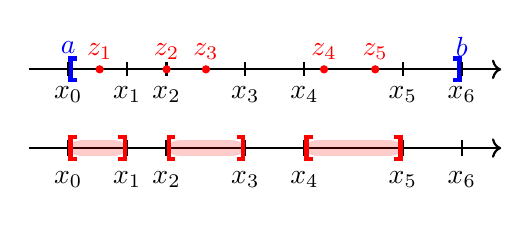
\begin{tikzpicture}[scale=5]
				
				% Draw the first numberline.
				\draw[->, thick] (-0.1,0) -- (1.1,0);
				
				% Draw the second numberline.
				\draw[->, thick] (-0.1,-.2) -- (1.1,-.2);
				
				% Draw the endpoints of the [a, b] interval.
				%\draw[ultra thick, blue] (0.02,-.02) -- (0.006,-.02) -- (0.006,.02) -- (0.02,.02) node at (0.006, .045) {$a$};
				%\draw[ultra thick, blue] (0.98,-.02) -- (0.994,-.02) -- (0.994,.02) -- (0.98,.02) node at (0.994, .045) {$b$};
				\draw[Bracket-, ultra thick, blue] (0,0) -- (0.01,0) node at (0, .055) {$a$};
				\draw[-Bracket, ultra thick, blue] (0.99,0) -- (1,0) node at (1, .058) {$b$};
				
				% Draw the subivision points.
				\foreach \x/\xtext in {0/$x_0$, 0.15/$x_1$, 0.25/$x_2$, 0.45/$x_3$, 0.6/$x_4$, 0.85/$x_5$, 1/$x_6$}{
					\draw[thick] (\x,0.5pt) -- (\x,-0.5pt) node[below] {\xtext};
					\draw[thick] (\x,-.22 ) -- (\x,-0.18 ) node at (\x, -0.28) {\xtext};
				}
				
				% Draw the subivision points.
				\foreach \x/\y in {0/0.15, 0.25/0.45, 0.6/0.85}{
					\draw[Bracket-, ultra thick, red] (\x,-.2) -- (\x + 0.01,-.2);
					\draw[-Bracket, ultra thick, red] (\y - 0.01,-.2) -- (\y,-.2);
					\fill[opacity = 0.2, red, rounded corners=1ex] (\x,-.22) -- (\y,-.22) --(\y,-.18) -- (\x,-.18) -- cycle;
				}
				
				% Draw the points of A_\delta.
				\foreach \x/\xtext in {0.08/$z_1$, 0.25/$z_2$, 0.35/$z_3$, 0.65/$z_4$, 0.78/$z_5$}{
					\fill[red] (\x,0pt) circle (0.3pt) node[above] {\xtext};	
				}
				
			\end{tikzpicture}
			\captionof{figure}{Az \( \mathcal{I} \) halmaz szemléltetése.}%
			\label{fig:felosztás-szakadás-szemléltetés}
				
			\begin{itemize}
				\item A felosztás: \( \tau = \{ x_0, \dots, x_6 \} \).
				\item A szakadások: \( A_\delta = \{ z_1, \dots, z_5 \} \).
				\item \( \mathcal{I} = \bigl\{ [x_0, x_1], \ [x_2, x_3], \ [x_4, x_5] \bigr\} \).
			\end{itemize}
		}[-6\baselineskip]
		amik a belsejükben tartalmaznak \( A_\delta \)-beli pontot (lásd \ref{fig:felosztás-szakadás-szemléltetés}. ábra), azaz
		\[
			\mathcal{I} \coloneq
			\setc[\Big]{ J \in \mathcal{F}(\tau) }{ \inter(J) \cap A_\delta \neq \emptyset }.
		\]
		Világos, hogy ekkor \( \tau \cup \mathcal{I} \) lefedi az \( A_\delta \) halmazat.
		Továbbá%
		\sidenote[][4\baselineskip]{%
			Mivel adott \( J \in \mathcal{I} \) intervallumhoz 
			van olyan \( z \in A_\delta \) szakadási pont, hogy
			\[
				z \in \inter(J)
				\quad \text{ és } \quad
				o_z(f) > \delta,
			\]
			ezért elmondható az alábbi becslés:
			\[
				\mathcal{O}(f, J) \geq o_z(f) > \delta.
			\]
		}
		\[
			\varepsilon	>
			\omega(f, \tau) =
			\sum_{I \in \mathcal{F}(\tau)} \mathcal{O}(f, I) {\cdot} \abs{I} \geq
			\sum_{J \in \mathcal{I}} \mathcal{O}(f, J) {\cdot} \abs{J} \geq
			\sum_{J \in \mathcal{I}} \delta {\cdot} \abs{J}.
		\]
		Következésképpen az \( \mathcal{I} \)-beli intervallumok hosszösszege így becsülhető:
		\[
		%	\sum_{J \in \mathcal{I}} \delta {\cdot} \abs{J} < \varepsilon
		%	\quad \iff \quad
			\sum_{J \in \mathcal{I}} \abs{J} < \frac{\varepsilon}{\delta}.
		\]
		Mivel \( \tau \) véges halmaz, ezért nullamértékű. 
		Következésképpen minden \( z \in \tau \) osztóponthoz hozzárendelhető 
		egy olyan \( J_z \subset \R \) intervallum, amellyel
		\[
			\tau \subset \bigcup_{z \in \tau} J_z
			\quad \text{ és } \quad
			\sum_{z \in \tau} \abs{J_z} < \varepsilon.
		\]
		Összességében elmondható, hogy
		\[
			A_\delta \,\subseteq\,
			\mathcal{I} \cup
		%	\mathopen{\raisebox{-0.9ex}{$ \biggl( $}}\,
			\bigcup_{z \in \tau} J_z
		%	\mathopen{\raisebox{-0.9ex}{$ \biggr) $}} 
			\quad \text{ és } \quad
		%	\sum_{z \in \tau} \abs{J_z}
			\sum_{z \in \tau} \abs{J_z} + \sum_{J \in \mathcal{I}} \abs{J} <
			\varepsilon + \frac{\varepsilon}{\delta} =
			\varepsilon \biggl( 1 + \frac{1}{\delta} \biggr).
		\]
		Ez pedig pontosan azt jelenti, hogy az \( A_\delta \) halmaz nullamértékű.
		
		\newpage
		
		\Backifstep
		Most legyen az \( \mathcal{A}_f \) halmaz nullamértékű. 
	%	Ekkor tetszőleges \( \delta > 0 \) esetén \( A_\delta \) is nullamértékű.
		Ekkor tetszőleges \( \varepsilon > 0 \)-hoz van olyan 
		\( I_n \subset \R \) korlátos és zárt intervallumsorozat \( (n \in \N) \), amellyel%
		%
		\sidenote[][0pt]{%
			Emlékeztetés gyanánt, ha \( x \in [a, b] \):
			\[
				x \in \mathcal{A}_f
				\quad \iff \quad
				f \notin \ContAt{x}.
			\]
		}
		\[
			\mathcal{A}_f \subseteq \bigcup_{n=0}^{\infty} \inter( I_n )
			\quad \text{ és } \quad
			\sum_{n = 0}^{\infty} \abs{ I_n } < \varepsilon.
		\]
		Ha pedig \( x \in [a, b] \) folytonossági pontja \( f \)-nek, 
		akkor \aref{lem:lokális-oszcillációs-és-folytonosság} lemma alapján
		\[
			f \in \ContAt{x} \quad \iff \quad o_x(f) = 0.
		\]
		Így a lokális oszcilláció jelentése miatt van olyan \( J_x \subset \R \) intervallum, hogy
		\[\label{eq:oszcilláció-felső-becslése}
			x \in \inter(J_x), \quad
			\mathcal{O}(J_x, f) = 
			\sup \Bigl\{ \abs\big{ f(u) - f(v) } \,\colon\, u, v \in J_x \cap [a, b] \Bigr\}
			< \varepsilon.
			\tag{\( * \)}
		\]
		Ezek alapján könnyen megadhatunk egy lefedését az \( [a, b] \) intervallumra%
		\sidenote[][0pt]{
			Tehát az \( f \)-nek minden szakadási és 
			nem szakadási pontját lefedjük a fenti halmazok segítségével. Itt
			\[
				\mathcal{A}^c_f = [a, b] \setminus \mathcal{A}_f.
			\]
		}
		\[
			[a, b] \subset 
			\Biggl(\, \bigcup_{n=0}^{\infty} \inter I_n  \Biggr) \cup
			\bigggl(\, \bigcup_{x \in \mathcal{A}_f^c} \inter J_x \bigggr).
		\]
		Ugyanakkor a \hyperref[lem:borel-lefedés]{Borel-lemma} alapján az előbbi nyílt lefedésből kiválasztatunk
		olyan véges \( A \subset \N \) és \( B \subset \mathcal{A}_f^c \) halmazokat, 
		amelyekkel szintén lefedhetjük az \( [a, b] \) intervallumot az alábbi módon:
		\[
			[a, b] \subset 
			\mathopen{\raisebox{-0.9ex}{$ \biggl( $}}\,
			\bigcup_{n \in A} \inter I_n
			\mathopen{\raisebox{-0.9ex}{$ \biggr) $}} 
			\ \cup \
			\mathopen{\raisebox{-0.9ex}{$ \biggl( $}}\,
			\bigcup_{x \in B} \inter J_x
			\mathopen{\raisebox{-0.9ex}{$ \biggr) $}}.
		\]
		Most vezessük be azt a \( \tau \subset [a, b] \) felosztást, 
		ami az \( I_n, J_x \ (n \in A,\, x \in B) \) intervallumok végpontjait 
		és az \( a, b \) számokat tartalmazza. Ekkor az
		\begin{alignat*}{6}
			U &\coloneq \Bigl\{ 
				&& & I &\in \mathcal{F}(\tau) \ \Big\vert \ && & I &\subseteq I_n &&\quad (n \in A) 
			\Bigr\} \\
			%		
			V &\coloneq 
			\Bigl\{ 
				&& & J &\in \mathcal{F}(\tau) \ \Big\vert \ && & J &\subseteq J_x &&\quad (x \in B) 
			\Bigr\}
		\end{alignat*}
		osztásintervallumoknak (a nem feltétlenül diszjunkt) szétosztását tekintve
		\[
			\omega(f, \tau) = 
			\sum_{I \in \mathcal{F}(\tau)} \mathcal{O}(I, f) {\cdot} \abs{I} \leq
			\sum_{I \in U} \mathcal{O}(I, f) {\cdot} \abs{I} + 
			\sum_{J \in V} \mathcal{O}(J, f) {\cdot} \abs{J}.
		\]
		Mivel feltettük, hogy az \( f \) korlátos, ezért egy alkalmas \( C \geq 0 \) számmal%
%		Mivel az \( f \) korlátos, ezért van olyan \( C \geq 0 \) szám, 
%		hogy minden \( I \subseteq [a, b] \) intervallumra
		%
		\sidenote[][0pt]{%
			A háromszög-egyenlőtlenség alapján
			\begin{align*}
				\mathcal{O}(I, f)
				&=    \sup \Bigl\{ \abs\big{f(x) - f(y)} \,\colon\, x, y \in I \Bigr\} \\
				&\leq \sup \Bigl\{ \abs\big{f(x)} + \abs\big{f(y)} \,\colon\, x, y \in I \Bigr\} \\
			%	&\leq \sup \Bigl\{ 2C \,\colon\, x, y \in I \Bigr\} \\
				&\leq 2C.
			\end{align*}
		}
		\[
			\abs\big{f(x)} \leq C \quad \bigl( x \in [a, b] \bigr)
			\qquad \Longrightarrow \qquad
			\smash{\uwave{\mathcal{O}(I, f) \leq 2C}} \quad (I \in U).
		\]
		Ennek és a \eqref{eq:oszcilláció-felső-becslése}-os becslésnek a felhasználásával kapjuk, hogy
		\begin{align*}
			\omega(f, \tau) &\leq 
		%	\sum_{I \in U} O_I (f) {\cdot} \abs{I} + 
		%	\sum_{J \in V} O_J (f) {\cdot} \abs{J} \leq
			\sum_{I \in U} 2C          {\cdot} \abs{I} + 
			\sum_{J \in V} \varepsilon {\cdot} \abs{J}   \leq
			2C          \cdot \sum_{n=0}^{\infty} \abs{I_n} + 
			\varepsilon \cdot \sum_{\mathclap{J \in \mathcal{F}(\tau)}} \abs{J} \\[3pt] &<
			2C \varepsilon + \varepsilon (b - a) =
			\smash{\uwave{\varepsilon ( 2C + b - a )}}.
		\end{align*}
		Következésképpen \( f \in \Riem{[a, b]} \).
	\end{proof}
	\begin{note}
		A Lebesgue-kritérium csak korlátos függvényre alkalmazható, hiszen
		\[
			\func{f}{[0, 1]}{\R}, \qquad
			f(x) \coloneq
			\left\{
			\begin{aligned}
				1/x, & \quad \text{ha } x \neq 0, \\
				0,  & \quad \text{ha } x = 0
			\end{aligned}
			\right.
		\]
		egyedül a nullában nem folytonos, de \( f \) nem Riemann-integrálható 
		(lásd \ref{fig:nem-korlátos-m-m-folytonos}. ábra).
		\marginnote{
			\centering
			\begin{tikzpicture}[scale=0.7]
				\begin{axis}[
					axis lines = middle,
					font=\large,
					xlabel = $x$,
					ylabel = $y$,
					xlabel style={xshift=75pt, yshift=-6pt},
					ylabel style={xshift=-7pt, yshift=60pt},
					domain=0.05:1,  % Starting from a small positive value to avoid division by 0
					samples=100,
					restrict y to domain=0:20,
					enlarge y limits = true,
					]
					
					% Plot for the function 1/x (for x > 0)
					\addplot[ultra thick, blue] {1/x};
					
					% Adding a point at the origin (0, 0) 
					\addplot[only marks, blue, ultra thick] coordinates {(0, 0)};
				\end{axis}
			\end{tikzpicture}
			\captionof{figure}{Az \( f \) függvény grafikonja.}\label{fig:nem-korlátos-m-m-folytonos}
		}[-10\baselineskip]
	\end{note}
\end{document}